\artikel{Archiv: Grieschiche Buchstaben}
{Na, wer weiß, der wievielte Buchstabe das ist? Ok, wir verraten es. Es ist
    bereits die 7. Folge unser aller Lieblingssammelfolgen. Wir danken allen
    Sammlern für ihr Vertrauen und wünschen weiterhin frohes Ausschneiden und
    Tauschen!}
{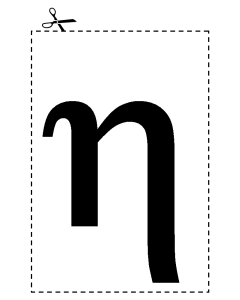
\includegraphics[width=\columnwidth]{grafik/eta}

    \paragraph{Verwendung}~\newline
    Mathematiker verwenden das $\eta$ gerne, wie sie ja eigentlich sowieso jeden
    griechischen Buchstaben verwenden. Dieser sieht aber ein bisschen so aus wie
    das y, daher wird beispielsweise $y - \eta$ und $z - \zeta$ (hatten wir letzte Folge)
    geschrieben.

    Aber nicht nur Hilfswissenschaftler bedienen sich gerne des $\eta$, auch die
    gefährliche Naturwissenschaft Physik beschreibt mit Hilfe dieses schönen
    Buchstabens die dynamische Viskosität, das ist die Fließfähigkeit bzw. die
    Zähflüssigkeit. Starker Kaffee hat beispielsweise eine große Viskosität.

    Die Physiker haben auch das Meson entdeckt und ihm den Buchstaben $\eta$ verpasst.
    Ein Meson ist ein Teilchen mittlerer Masse, das sich zwischen dem schweren
    Proton und dem leichten Elektronengewicht aufhält. Quasi mittelstarker Kaffee.

    Der Wirkungsgrad, also das Verhältnis von Nutzen und Aufwand, wird auch mit
    $\eta$
    bezeichnet. Bei Maschinen und Wärmequellen kann man das beispielsweise
    berechnen, die Formel dafür ist auch gar nicht mal so schwer: Leistung mal
    Zeit. Schneller Kaffee kochen, mehr Kaffee trinken.

    Erstmals machen auch Bauingenieure von einem Buchstaben gebrauch, das $\eta$
    bezeichnet den Sicherheitsbeiwert. Das ist das, was die Ingenieure
    sicherheitshalber noch mal draufpacken, damit nix kaputtgeht. Analogon: lieber
    einen Löffel Kaffee mehr.
    \paragraph{Zubereitung}~\newline
    Das $\eta$ ist so ein Zwischending zwischen n und y. Zum Zubereiten zuerst ein n
    zeichnen und dann kurz vor dem Ende des zweiten Beins zum y umschwenken. So
    einfach geht das.
    \paragraph{Empfehlung}~\newline
    Da der Buchstabe schön aussieht und einfach zuzubereiten ist, empfehlen wir
    häufige Anwendung. Aber andere Buchstaben darüber nicht vernachlässigen!
    Nächstes Mal gibt es übrigens wieder einen der begehrten und beliebten
    Doppelbuchstaben: $\theta$ und $\Theta$}
{Arne Pottharst}


Dieser Artikel erschien ursprünglich im Juni 2006 und steht daher nicht unter
CC-BY-SA.
